\subsection{Defining the Robot’s Shape: Square, Circular, Polygonal or Triangular Designs}

Following the decisions on movement type and wheel configuration, another crucial design consideration was the \textbf{shape} of the robot's base. The geometry of the robot directly affects not only its aesthetic but also its \textbf{manoeuvrability}, \textbf{stability}, \textbf{sensor placement} and \textbf{ability to navigate tight indoor spaces}. The primary shapes considered were \textbf{square}, \textbf{circular}, \textbf{polygonal} and \textbf{triangular} forms, each offering distinct advantages and challenges.

\begin{itemize}
    \item \textbf{Square:} Symmetry, ease of design, but corners can get caught and less smooth navigation.
    \item \textbf{Circular:} Excellent manoeuvrability, ideal for dynamic environments, but less space-efficient and more complex to construct.
    \item \textbf{Polygonal:} Balance between round and angular, unique structural advantages, but more complex to design and assemble.
    \item \textbf{Triangular:} Compact, simple three-wheel integration, but limited stability and challenging payload distribution.
\end{itemize}

\subsection{Group Cardboard Prototype Proposals}

When tasked with creating a cardboard prototype of the module, the group presented four different design proposals with detailed analysis of their advantages and disadvantages.

\subsubsection{Omnidirectional robot with four wheels positioned at the vertices of a square}

\textbf{Proposed by:} Ermelinda Giulivo

\begin{figure}[H]
    \centering
    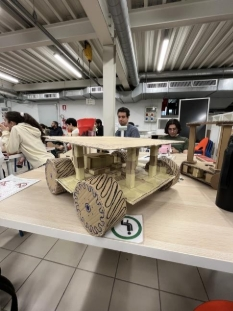
\includegraphics[width=0.5\linewidth]{../ReportMovementModule/images/Aspose.Words.728084da-df58-4b9d-a372-f65cffbdb23d.002.jpeg}
    \caption{Square-based Omnidirectional Robot}
\end{figure}

\begin{table}[H]
\centering
\begin{tabular}{|p{0.45\textwidth}|p{0.45\textwidth}|}
\hline
\multicolumn{2}{|c|}{\textbf{Omnidirectional robot with four wheels positioned at the vertices of a square}} \\
\hline
\textbf{Pros} & \textbf{Cons} \\
\hline
\textbf{Excellent Stability:} The square layout provides a wide and balanced support base, enhancing stability, especially when carrying payloads or navigating uneven indoor floors. & \textbf{Larger Turning Radius Compared to Circular Robots:} Although it can strafe and rotate, the square footprint is bulkier when fitting into very tight or irregularly shaped spaces. \\
\hline
\textbf{Full Omnidirectional Mobility:} With wheels positioned symmetrically, the robot can move smoothly in any direction — forward, backward, sideways or diagonally — without needing to rotate first. & \textbf{Wheel Synchronization Complexity:} Precise control of all four wheels is essential. Small discrepancies in motor performance can cause drift or errors in movement if not properly calibrated. \\
\hline
\textbf{Simple Mechanical Symmetry:} The square design makes mechanical construction easier and ensures even distribution of forces, reducing stress on the frame. & \textbf{Higher Energy Consumption:} Coordinated omnidirectional movement (especially diagonal motion) can be less energy-efficient compared to simpler drive systems. \\
\hline
\textbf{Good for Sensor Placement:} The square chassis offers clear and logical positions for sensors, allowing for easy 360-degree coverage with minimal blind spots. & \textbf{Cost and Mechanical Complexity:} Four omni-wheels and corresponding motors, encoders and controllers increase system cost and complexity compared to simpler two-wheel or three-wheel robots. \\
\hline
\textbf{Predictable and Balanced Control:} Because of the symmetry, the control algorithms (e.g., for velocity distribution across wheels) can be simpler and more consistent. & \textbf{Vulnerability to Wheel Slippage:} Omni-wheels rely on small rollers, which can slip on smooth or dusty indoor surfaces, potentially affecting localization accuracy. \\
\hline
\end{tabular}
\end{table}

\subsubsection{Triangular-shaped, three-wheel omnidirectional robot}

\textbf{Proposed by:} Rafael Monllor Ballesteros

\begin{figure}[H]
    \centering
    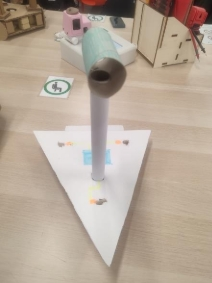
\includegraphics[width=0.5\linewidth]{../ReportMovementModule/images/Aspose.Words.728084da-df58-4b9d-a372-f65cffbdb23d.003.jpeg}
    \caption{Triangular-shaped Omnidirectional Robot}
\end{figure}

\begin{table}[H]
\centering
\begin{tabular}{|p{0.45\textwidth}|p{0.45\textwidth}|}
\hline
\multicolumn{2}{|c|}{\textbf{Triangular-shaped, three-wheel omnidirectional robot}} \\
\hline
\textbf{Pros} & \textbf{Cons} \\
\hline
\textbf{Compact Design:} Three wheels in a triangular configuration create an optimally compact base while still maintaining stability. & \textbf{Lower Weight Distribution Stability:} Compared to four-wheel designs, triangular bases provide less stability for tall or top-heavy constructions. \\
\hline
\textbf{Less Mechanical Complexity:} One fewer motor and wheel compared to four-wheel designs means fewer components to maintain, calibrate, and potentially fail. & \textbf{More Complex Control Algorithms:} Achieving precise omnidirectional movement with three wheels can require more sophisticated software than four-wheel configurations. \\
\hline
\textbf{Lower Power Consumption:} Operating three motors instead of four reduces total energy usage, potentially extending battery life. & \textbf{Potential Payload Limitations:} The triangular base may support less weight or require more careful weight distribution than square configurations. \\
\hline
\textbf{Efficient for Small Robots:} Ideal for light-duty applications where high payload capacity is not necessary. & \textbf{Less Redundancy:} If one motor or wheel fails, the robot's ability to move properly is much more compromised than with four-wheel designs. \\
\hline
\end{tabular}
\end{table}

\subsubsection{Polygonal-shaped omnidirectional robot with four wheels arranged in a cross configuration}

\textbf{Proposed by:} Daniel Mauricio Ruiz Suarez

\begin{figure}[H]
    \centering
    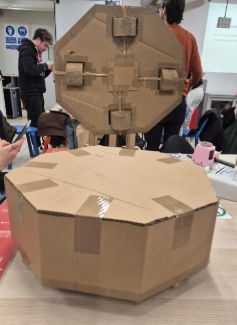
\includegraphics[width=0.5\linewidth]{../ReportMovementModule/images/Aspose.Words.728084da-df58-4b9d-a372-f65cffbdb23d.004.jpeg}
    \caption{Polygonal-shaped Robot with Cross Wheel Configuration}
\end{figure}

\begin{table}[H]
\centering
\begin{tabular}{|p{0.45\textwidth}|p{0.45\textwidth}|}
\hline
\multicolumn{2}{|c|}{\textbf{Polygonal-shaped omnidirectional robot with four wheels arranged in a cross configuration}} \\
\hline
\textbf{Pros} & \textbf{Cons} \\
\hline
\textbf{Optimized Use of Space:} The polygonal chassis (such as hexagonal or octagonal) better fits the cross pattern while allowing more efficient internal layout of components compared to a purely circular design. & \textbf{Design Complexity:} More complicated to design and assemble compared to pure circular or square robots. \\
\hline
\textbf{Simplified Path Planning:} Because the wheels are symmetrically arranged, control algorithms for movement and localization become more predictable and manageable. & \textbf{Potential for Increased Size:} Depending on the polygon shape and wheel placement, the overall footprint of the robot could become larger than necessary for tight indoor environments. \\
\hline
\textbf{Better Obstacle Navigation:} The extended wheel positions can help in negotiating tight spaces or approaching obstacles at different angles more smoothly. & \textbf{Higher Control Precision Needed:} Maintaining synchronized wheel movement across a cross configuration demands precise motor control to avoid unwanted drift or vibration, especially at higher speeds. \\
\hline
\textbf{Load Distribution Sensitivity:} Uneven weight distribution can negatively affect movement performance, as each wheel may bear different loads during turns or fast translations. & \\
\hline
\end{tabular}
\end{table}

\subsubsection{Circular-shaped, three-wheel omnidirectional robot}

\textbf{Proposed by:} Jurij Diego Scandola

\begin{figure}[H]
    \centering
    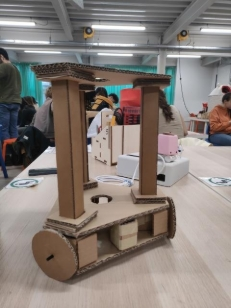
\includegraphics[width=0.5\linewidth]{../ReportMovementModule/images/Aspose.Words.728084da-df58-4b9d-a372-f65cffbdb23d.005.jpeg}
    \caption{Circular-shaped Omnidirectional Robot}
\end{figure}

\begin{table}[H]
\centering
\begin{tabular}{|p{0.45\textwidth}|p{0.45\textwidth}|}
\hline
\multicolumn{2}{|c|}{\textbf{Circular-shaped, three-wheel omnidirectional robot}} \\
\hline
\textbf{Pros} & \textbf{Cons} \\
\hline
\textbf{Excellent Manoeuvrability:} The circular design eliminates corners, allowing smooth and uninterrupted movement and rotation in any direction — ideal for navigating tight, cluttered indoor environments. & \textbf{Reduced Structural Simplicity:} Building a strong, circular chassis (especially with flat materials like cardboard or sheet metal) can be mechanically more complex compared to square or polygonal shapes. \\
\hline
\textbf{Compact and Symmetrical:} The circular form naturally distributes mass and components around the centre, enhancing balance and improving dynamic stability during motion. & \textbf{Lower Load Capacity:} Three-wheel setups naturally provide less stability and support for heavy loads compared to four-wheel configurations and the circular frame can limit internal mounting options for large or heavy components. \\
\hline
\textbf{Efficient for Omnidirectional Control:} The 120° placement of the three wheels around the circle simplifies omnidirectional movement algorithms and ensures consistent movement performance. & \textbf{Challenging Internal Layout:} Fitting rectangular or square components (like batteries, boards, and sensors) inside a circular space can be inefficient and may lead to wasted internal volume. \\
\hline
\textbf{Minimal Risk of Snagging:} Without edges or corners, the robot can more easily avoid getting caught on obstacles, furniture, or tight doorways. & \textbf{Sensitivity to Weight Imbalance:} Proper balancing is critical; even slight asymmetry in weight distribution can significantly impact the robot's movement precision and stability. \\
\hline
\textbf{Aesthetically Appealing:} The circular shape often results in a cleaner, more modern appearance, which can be a factor in user-facing or commercial applications. & \textbf{Less Redundancy:} With only three wheels, if one wheel or motor fails, the robot's mobility is seriously compromised compared to a four-wheel design. \\
\hline
\end{tabular}
\end{table}

\subsection{Selected Approach}

After evaluating all prototype designs, the group decided on a modified polygonal approach that incorporated a \textbf{dodecagonal (12-sided) base} with \textbf{three omnidirectional wheels} arranged in a triangular configuration. This combined the stability advantages of a wide base with the mechanical simplicity of a three-wheel system.

\begin{figure}[H]
    \centering
    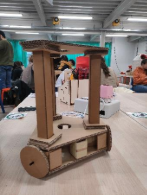
\includegraphics[width=0.5\linewidth]{../ReportMovementModule/images/Aspose.Words.728084da-df58-4b9d-a372-f65cffbdb23d.006.png}
    \caption{Final Cardboard Prototype}
\end{figure}

This approach offered several advantages:
\begin{itemize}
    \item The polygonal shape approximated a circle for smooth navigation while being easier to fabricate from flat materials
    \item Using three wheels reduced complexity and power consumption compared to four-wheel designs
    \item The wide base provided good stability without excessive weight
    \item The design allowed for sensor placement around the perimeter with minimal blind spots
    \item The balanced triangular wheel arrangement facilitated simple yet effective omnidirectional control
\end{itemize}

These early tests helped us set a clearer direction for both technical and conceptual development, bridging the gap between idea and implementation.
